%---
\section{Material Assays}
\label{sec:Materials}

Trace radioactivity in detector materials can be a dominant background for the direct dark-matter searches. In addition to this bulk contamination, a major source of background can be caused by the cosmogenic activation of the materials and by the surface contamination (due to radon diffusion and plate out of the radon daughters produced in the surrounding air).
Beta and alpha particles produced by the radionuclide decays can typically contribute to the background only if the atom is in contact with the \LAr\,target, while gammas and neutrons, the last ones from spontaneous fission and $(\alpha,n)$ interactions, can produce background from more distant sites.

A strategy for selecting the materials, as well as machining, storing, transporting and mounting the detector components, is mandatory in order to control the backgrounds and to maximize the physics reach of \DSks. This will be accomplished by developing the ``background budget'' to identify materials' purity requirements. In addition to the assays on the raw purchased materials, performed to identify the right technologies and compositions, we are developing cleaning and handling procedures to meet radiopurity standards, and performing assays to validate processes for the construction and commissioning of the detector and its components.

In \DSks\,this responsibility is delegated to the Materials and Assays Working Group (\MAWG), a single Working Group within the collaboration, comprised of experts in each of the assay methods and representatives from each institution that hosts assay capabilities. The group coordinates and schedules the assays according to the pre-evaluated radiopurity requirements, the urgency, the capacity of the available assaying resources and their queue.

The goal is to assay and approve {\it all} materials or items selected to reside within the cryostat, particularly by scrutinizing the entire $^{232}$Th and $^{238}$U decay chains. This calls for multiple assays with multiple techniques for each sample, as different techniques are applicable to different sub-chains of the $^{232}$Th and $^{238}$U decay chains. These results are combined with the $(\alpha,n)$ cross-sections, calculated according to the chemical composition of the material in order to extract the neutron yield expected in the detector.


%---
\subsection{Radio-purity database}
\label{sec:Mat-DB}

The need for fast access to, and exchange of data between different Working Groups (WG) is addressed by the DarkSide Materials Database (MDB). Information on the radioactive content of materials to be used for \DSks\,construction is stored therein, and is crucial for the comprehensive estimation of the background budget for the experiment. The MDB contains all the relevant information about samples: chemical composition, origin (production batch), data-sheets, pictures, part of the detector where it will be placed, history of assays etc. This information is included in the total background budget estimation and carefully evaluated. Rules for handling and cleaning of samples, developed and verified during the screening process, are also stored in the database. Later, during the detector construction and integration, reproducible results of the estimated internal background may be expected upon application of the provided handling and cleaning procedures.

The database helps to systematize the radioactive background budget estimation, material selection and tracking, assay prioritization, and cleaning and handling methods. Additionally, the database is also used to balance the workload and assay resources between numerous institutions involved in the task by coupling assay needs with assay capabilities of members of the Materials WG.

\begin{figure*}[!t]
\center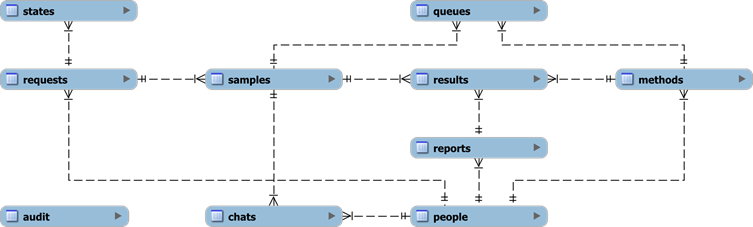
\includegraphics[width=\textwidth]{./Figures/mdb_structure.png}
\caption[\DSks\ materials database structure]{A simplified \DSks\ materials database structure. Information on each relevant aspect of the assay process is stored in the database, facilitating the management of the whole assay process.}
\label{fig:mdb_structure}
\end{figure*} 

The MDB structure reflects the flow of the material assay process, aiding material selection and application during the construction phase of the experiment. The database consists of several cross-related tables, holding information on the status of the assay requests, screening methods, samples, assay results and people (institutions) involved (see Fig.~\ref{fig:mdb_structure}). It also keeps track of the queues in different facilities, and the history and the current status of any assay performed within the \MAWG. A convenient web-based interface is provided for the users (see Fig.~\ref{fig:mdb_results}), dedicated to: ease submission of new assay requests from other Working Groups; browse and report of the assay results (including uploading the results); and to manage the assay status of the samples and queues at different facilities.

\begin{figure*}[!t]
\center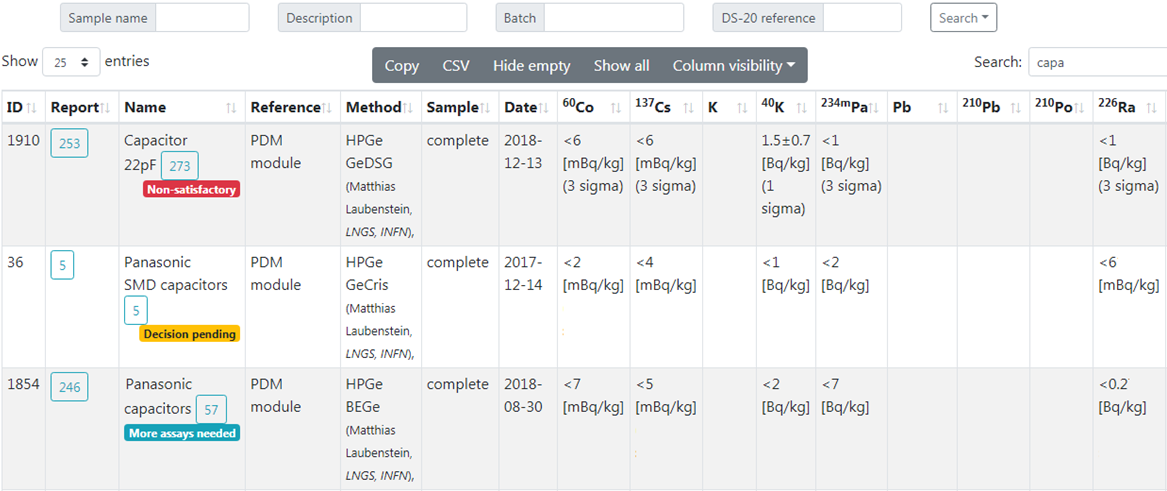
\includegraphics[width=\textwidth]{./Figures/mdb_results.png}
\caption[Web interface of \DSks\ materials database]{Interface web page, presenting a selection of assay results for various types of capacitors. The database is also used to manage the assay process of each sample.}
\label{fig:mdb_results}
\end{figure*} 

Assay results obtained for the materials used for \DSfs\,were also imported to the new database. Currently the database stores almost 2000 assay results (more than 120 assays performed since 2017) of nearly 300 samples, and counts (see Tab.~\ref{t:mdb_assays}). The \MAWG\ has established protocols to efficiently handle the radioactive budget of the experiment.


%---
\subsection{Managing Assay Capabilities}
\label{sec:MatAssay-RadiopurityManagement}

To ensure the radiopurity of all detector materials to the levels defined by the background model, the \MAWG\ has developed a radiopurity assay program that takes advantage of facilities throughout the collaboration. Overall, it is anticipated that this program will span approximately three years and will involve around a thousand more assays, including searches for radiopure materials, development and validation of cleaning and handling procedures, and screening of all detector components. The collaboration has extensive and diverse assay capabilities that are sufficient to complete this program on schedule, with extra capacity to handle additional unforeseen assays. Estimates of the capacity available to \DSks\ for each assay type are summarized in Tab.~\ref{t:mdb_estimate}. The assay challenges are organized into six focus areas: mass spectrometry (\ICPMS), radon emanation, direct gamma assay (HPGe), surface assays (alpha activity), cosmogenic activation and materials handling and process development.


%---
\subsection{Radioactive budget}
\label{sec:Mat-Bdg}

The radioactive budget states the expected background of everything that goes into the detector, taking into account material's (element) radiopurity, mass, composition, shape and location. These parameters are the input of Monte Carlo simulations, performed using a Geant4-based package written within the collaboration and called G4DS. The result of the simulation is the efficiency of our detector for rejecting the background coming from different sources, either because of geometrical reasons or because of active tagging of undesired events. The neutron budget is calculated on a single-element basis, so the mentioned inputs (radiopurity, composition and the position in the detector) are needed for every component of the detector.

The most critical requirement in terms of radiopurity is given by the $\alpha$ activity, mainly caused by the naturally occurring radioactive chains of $^{232}$Th and $^{238}$U and potentially producing neutrons through $(\alpha,n)$ reactions. The cross section of this reaction is calculated using the {\it neucbot} program, where the energy spectrum of neutrons is generated as well. Hence, the (chemical) composition and construction of each component needs to be known with sufficient detail in order to calculate the interaction cross-sections correctly.

Provided that some construction elements may be in similar locations, and that a component may  be used in different places, a cross-linked, multi-tab spreadsheet is used to calculate the expected neutron budget. Propagation of any modifications or updates in a coherent way is easy to maintain. A summary of background budget components is tabulated in a user-friendly form, collecting all the relevant information structured following the same organization scheme as the Working Groups in the collaboration (Veto, TPC, PhotoElectronics, etc). \MAWG\ is in close cooperation with other WGs through dedicated group representatives, aiding selection of proper construction materials at the early stages of the design. The background budget is constantly evolving and converging as the material assay campaign progresses, such that more components' activities are determined. It is estimated that over 1000 more assays will be performed until the completion of the detector construction, for more than 150 expected material samples.

\begin{table}[t!]
\center\begin{tabular}{lc}
\hline
\hline
Assay Method					&Number of assays\\
\hline 
\ICPMS							&50\\
Germanium spectroscopy			&40\\
Chemical extraction	of \ce{Po}	&20\\
Surface $\alpha$'s counting		&5\\
Radon emanation					&5\\
Other							&3\\
\hline 
\end{tabular}
\caption[Summary of \DSks\ assays performed]{Summary of the assays performed since~2017 in preparations of the \DSks\ construction, with breakdown by assay method.}
\label{t:mdb_assays}
\end{table} 

\begin{table}[!t]
\center\begin{tabular}{lc}
\hline\hline
\multirow{2}{*}{Assay Method}	&Capacity\\
								&[assays per year]\\
\hline
ICP-MS							&60\\
Germanium spectroscopy			&35\\
Chemical extraction	of \ce{Po}	&20\\
Surface $\alpha$'s counting		&10\\
Radon emanation					&10\\
\hline 
\end{tabular}
\caption[Summary of the assay capabilities available for \DSks]{Summary of the assay capabilities available for \DSks.}
\label{t:mdb_estimate}
\end{table}